%% This is the ctufit-thesis example file. It is used to produce theses
%% for submission to Czech Technical University, Faculty of Information Technology.
%%
%% Get the newest version from
%% https://gitlab.fit.cvut.cz/theses-templates/FITthesis-LaTeX
%%
%%
%% Copyright 2021, Eliska Sestakova and Ondrej Guth
%%
%% This work may be distributed and/or modified under the
%% conditions of the LaTeX Project Public Licenese, either version 1.3
%% of this license or (at your option) any later version.
%% The latest version of this license is in
%%  https://www.latex-project.org/lppl.txt
%% and version 1.3 or later is part of all distributions of LaTeX
%% version 2005/12/01 or later.
%%
%% This work has the LPPL maintenance status `maintained'.
%%
%% The current maintainer of this work is Ondrej Guth.
%% Contact ondrej.guth@fit.cvut.cz for bug reports.
%% Alternatively, submit bug reports into the tracker at
%% https://gitlab.fit.cvut.cz/theses-templates/FITthesis-LaTeX/issues
%%
%%

% arara: pdflatex
% arara: biber
% arara: pdflatex
% arara: pdflatex

%%%%%%%%%%%%%%%%%%%%%%%%%%%%%%%%%%%%%%%%%
% CLASS OPTIONS
% language: czech/english/slovak
% thesis type: bachelor/master/dissertation
% colour: bw for black&white OR no option for default colour scheme
% electronic or printed: oneside/twoside (default)
%%%%%%%%%%%%%%%%%%%%%%%%%%%%%%%%%%%%%%%%%
\documentclass[czech,bachelor,unicode,oneside]{ctufit-thesis}

%%%%%%%%%%%%%%%%%%%%%%%%%%%%%%%%%%
% FILL IN THIS INFORMATION
%%%%%%%%%%%%%%%%%%%%%%%%%%%%%%%%%%
\ctufittitle{Název příkladné závěrečné práce} % replace with the title of your thesis
\ctufitauthorfull{Michal Dobeš} % replace with your full name (first name(s) and then family name(s) / surname(s)) including academic degrees
\ctufitauthorsurnames{Dobeš} % replace with your surname(s) / family name(s)
\ctufitauthorgivennames{Michal} % replace with your first name(s) / given name(s)
\ctufitsupervisor{Ing.\,Jiří Hunka} % replace with name of your supervisor/advisor (include academic degrees)
\ctufitdepartment{Katedra softwarového inženýrství} % replace with the department of your defence
\ctufityear{2024} % replace with the year of your defence
\ctufitdeclarationplace{Praze} % replace with the place where you sign the declaration
\ctufitdeclarationdate{\today} % replace with the date of signature of the declaration
\ctufitabstractCZE{Fill in abstract of this thesis in Czech language. Class aptent taciti sociosqu ad litora torquent per conubia nostra, per inceptos hymenaeos. Cras pede libero, dapibus nec, pretium sit amet, tempor quis. Sed vel lectus. Donec odio tempus molestie, porttitor ut, iaculis quis, sem. Suspendisse sagittis ultrices augue.}
\ctufitabstractENG{Fill in abstract of this thesis in English language. Class aptent taciti sociosqu ad litora torquent per conubia nostra, per inceptos hymenaeos. Cras pede libero, dapibus nec, pretium sit amet, tempor quis. Sed vel lectus. Donec odio tempus molestie, porttitor ut, iaculis quis, sem. Suspendisse sagittis ultrices augue.}
\ctufitkeywordsCZE{enter, commma, separated, list, of, keywords, in, CZECH}
\ctufitkeywordsENG{enter, commma, separated, list, of, keywords, in, ENGLISH}
%%%%%%%%%%%%%%%%%%%%%%%%%%%%%%%%%%
% END FILL IN
%%%%%%%%%%%%%%%%%%%%%%%%%%%%%%%%%%

%%%%%%%%%%%%%%%%%%%%%%%%%%%%%%%%%%
% CUSTOMIZATION of this template
% Skip this part or alter it if you know what you are doing.
%%%%%%%%%%%%%%%%%%%%%%%%%%%%%%%%%%

\RequirePackage{iftex}[2020/03/06]
\iftutex % XeLaTeX and LuaLaTeX
    \RequirePackage{ellipsis}[2020/05/22] %ellipsis workaround for XeLaTeX
\else
    \RequirePackage[utf8]{inputenc}[2018/08/11] %this file encoding
    \RequirePackage{lmodern}[2009/10/30] % vector flavor of Computer Modern font
\fi

% hyperlinks
\RequirePackage[pdfpagelayout=TwoPageRight,colorlinks=false,allcolors=decoration,pdfborder={0 0 0.1}]{hyperref}[2020-05-15]

% uncomment the following to hide all hyperlinks
% \RequirePackage[pdfpagelayout=TwoPageRight,hidelinks]{hyperref}[2020-05-15]

\RequirePackage{pdfpages}[2020/01/28]

\setcounter{secnumdepth}{4} % numbering sections; 4: subsubsection



%%%%%%%%%%%%%%%%%%%%%%%%%%%%%%%%%%
% CUSTOMIZATION of this template END
%%%%%%%%%%%%%%%%%%%%%%%%%%%%%%%%%%


%%%%%%%%%%%%%%%%%%%%%%
% DEMO CONTENTS SETTINGS
% You may choose to modify this part.
%%%%%%%%%%%%%%%%%%%%%%
\usepackage{dirtree}
\usepackage{lipsum,tikz}
\usepackage{csquotes}
\usepackage[style=iso-numeric]{biblatex}
\addbibresource{text/bib-database.bib}
\usepackage{listings} % typesetting of sources
%\usepackage[newfloat]{minted}\captionsetup[listing]{position=top} % typesetting of sources

%theorems, definitions, etc.
\theoremstyle{plain}
\newtheorem{theorem}{Věta}
\newtheorem{lemma}[theorem]{Tvrzení}
\newtheorem{corollary}[theorem]{Důsledek}
\newtheorem{proposition}[theorem]{Návrh}
\newtheorem{definition}[theorem]{Definice}
\theoremstyle{definition}
\newtheorem{example}[theorem]{Příklad}
\theoremstyle{remark}
\newtheorem{note}[theorem]{Poznámka}
\newtheorem*{note*}{Poznámka}
\newtheorem{remark}[theorem]{Pozorování}
\newtheorem*{remark*}{Pozorování}
\numberwithin{theorem}{chapter}
%theorems, definitions, etc. END
%%%%%%%%%%%%%%%%%%%%%%
% DEMO CONTENTS SETTINGS END
%%%%%%%%%%%%%%%%%%%%%%

\begin{document} 
\frontmatter\frontmatterinit % do not remove these two commands

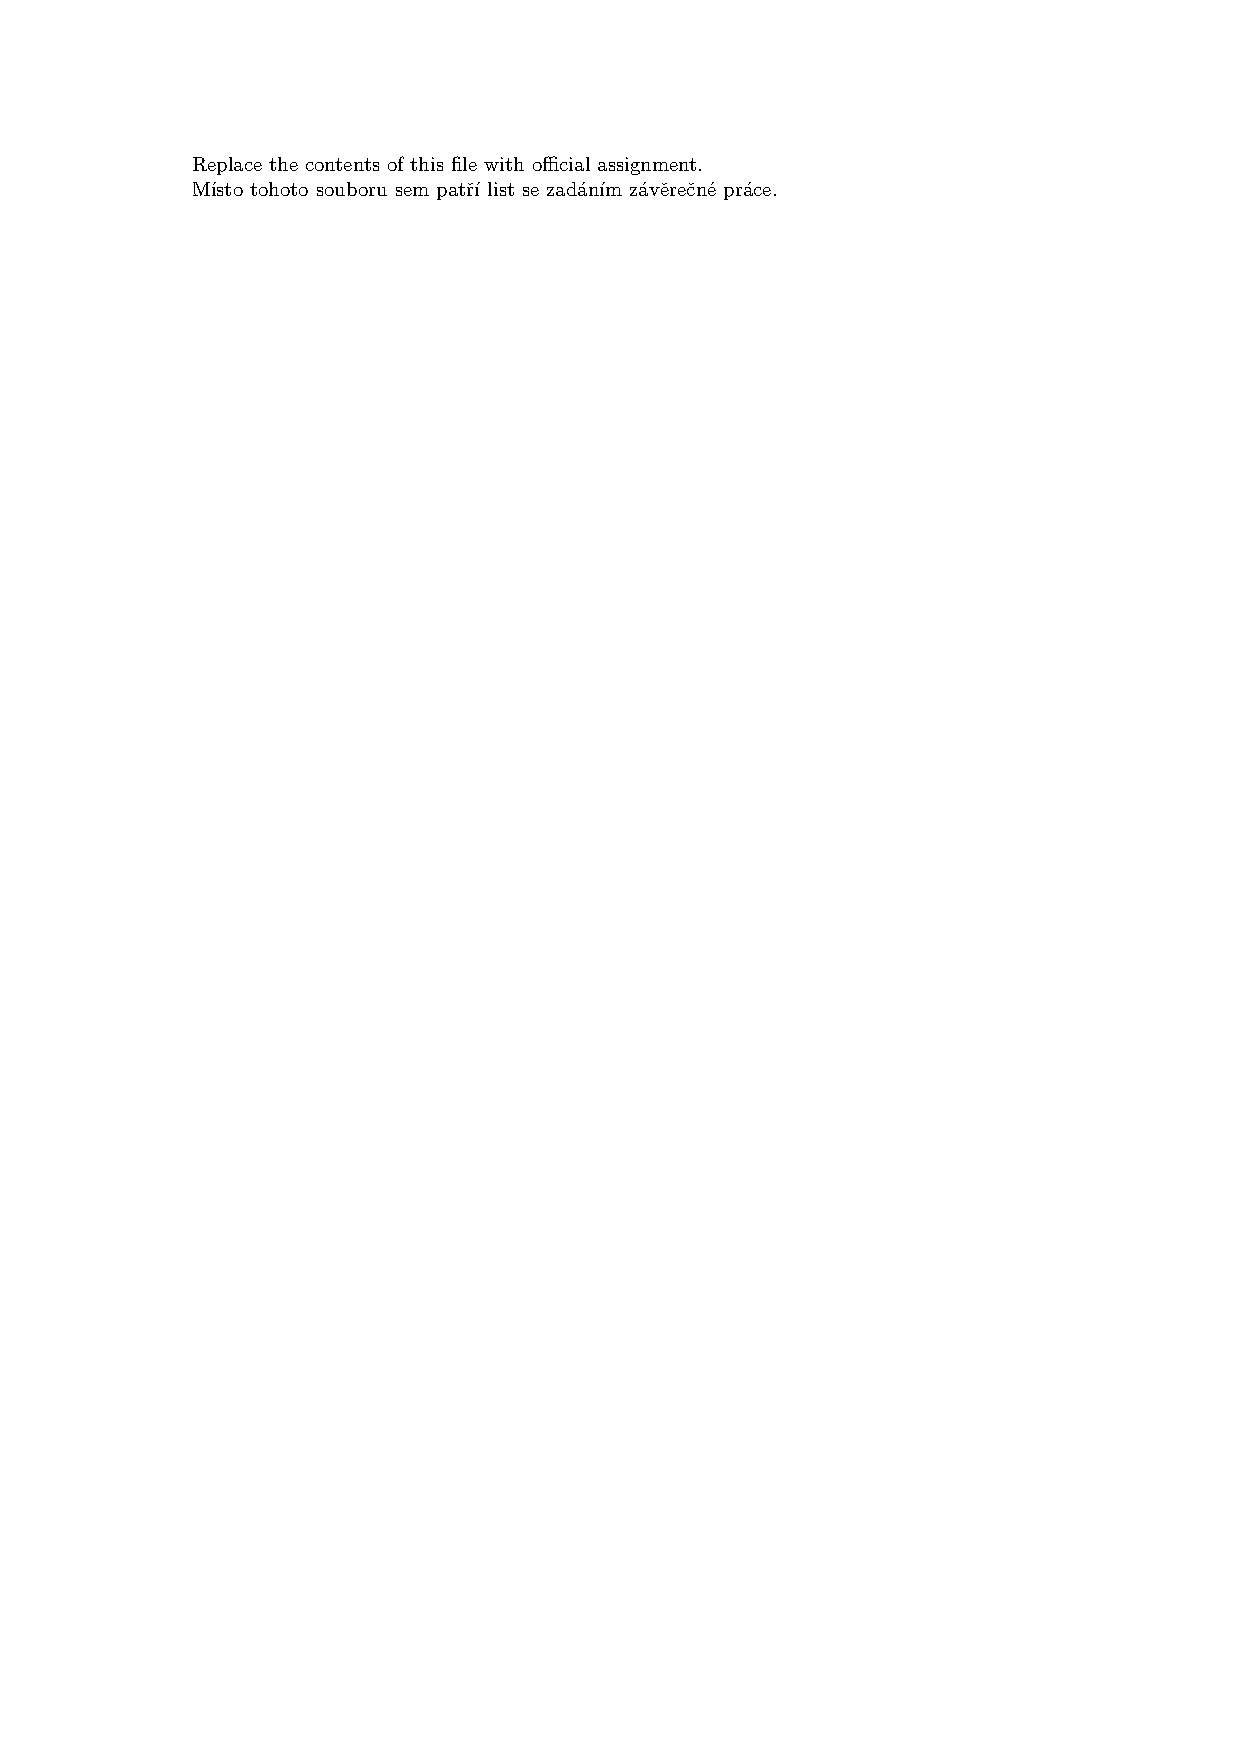
\includepdf[pages={1-}]{assignment-include.pdf} % replace that file with your thesis assignment provided by study office

\thispagestyle{empty}\cleardoublepage\maketitle % do not remove these three commands

\imprintpage % do not remove this command

\tableofcontents % do not remove this command
%%%%%%%%%%%%%%%%%%%%%%
% list of other contents: figures, tables, code listings, algorithms, etc.
% add/remove commands accordingly
%%%%%%%%%%%%%%%%%%%%%%
\listoffigures % list of figures
\begingroup
\let\clearpage\relax
\listoftables % list of tables
\lstlistoflistings % list of source code listings generated by the listings package
% \listoflistings % list of source code listings generated by the minted package
\endgroup
%%%%%%%%%%%%%%%%%%%%%%
% list of other contents END
%%%%%%%%%%%%%%%%%%%%%%

%%%%%%%%%%%%%%%%%%%
% ACKNOWLEDGMENT
% FILL IN / MODIFY
% This is a place to thank people for helping you. It is common to thank your supervisor.
%%%%%%%%%%%%%%%%%%%
\begin{acknowledgmentpage}
	Chtěl bych poděkovat především sit amet, consectetuer adipiscing elit. Curabitur sagittis hendrerit ante. Class aptent taciti sociosqu ad litora torquent per conubia nostra, per inceptos hymenaeos. Cras pede libero, dapibus nec, pretium sit amet, tempor quis. Sed vel lectus. Donec odio tempus molestie, porttitor ut, iaculis quis, sem. Suspendisse sagittis ultrices augue.
\end{acknowledgmentpage} 
%%%%%%%%%%%%%%%%%%%
% ACKNOWLEDGMENT END
%%%%%%%%%%%%%%%%%%%


%%%%%%%%%%%%%%%%%%%
% DECLARATION
% FILL IN / MODIFY
%%%%%%%%%%%%%%%%%%%
% INSTRUCTIONS
% ENG: choose one of approved texts of the declaration. DO NOT CREATE YOUR OWN. Find the approved texts at https://courses.fit.cvut.cz/SFE/download/index.html#_documents (document Declaration for FT in English)
% CZE/SLO: Vyberte jedno z fakultou schvalenych prohlaseni. NEVKLADEJTE VLASTNI TEXT. Schvalena prohlaseni najdete zde: https://courses.fit.cvut.cz/SZZ/dokumenty/index.html#_dokumenty (prohlášení do ZP)
\begin{declarationpage}
FILL IN ACCORDING TO THE INSTRUCTIONS. VYPLNTE V SOULADU S POKYNY. Lorem ipsum dolor sit amet, consectetuer adipiscing elit. Curabitur sagittis hendrerit ante. Class aptent taciti sociosqu ad litora torquent per conubia nostra, per inceptos hymenaeos. Cras pede libero, dapibus nec, pretium sit amet, tempor quis. Sed vel lectus. Donec odio tempus molestie, porttitor ut, iaculis quis, sem. Suspendisse sagittis ultrices augue. Donec ipsum massa, ullamcorper in, auctor et, scelerisque sed, est. In sem justo, commodo ut, suscipit at, pharetra vitae, orci. Pellentesque pretium lectus id turpis.

Lorem ipsum dolor sit amet, consectetuer adipiscing elit. Curabitur sagittis hendrerit ante. Class aptent taciti sociosqu ad litora torquent per conubia nostra, per inceptos hymenaeos. Cras pede libero, dapibus nec, pretium sit amet, tempor quis. Sed vel lectus. Donec odio tempus molestie, porttitor ut, iaculis quis, sem. Suspendisse sagittis ultrices augue. Donec ipsum massa, ullamcorper in, auctor et, scelerisque sed, est. In sem justo, commodo ut, suscipit at, pharetra vitae, orci. Pellentesque pretium lectus id turpis.
\end{declarationpage}
%%%%%%%%%%%%%%%%%%%
% DECLARATION END
%%%%%%%%%%%%%%%%%%%

\printabstractpage % do not remove this command

%%%%%%%%%%%%%%%%%%%
% SUMMARY
% FILL IN / MODIFY
% OR REMOVE ENTIRELY (upon agreement with your supervisor)
% (appropriate to remove in most theses)
%%%%%%%%%%%%%%%%%%%
% \begin{summarypage}
% \section*{Summary section}
% 
% \lipsum[1][1-8]
% 
% \section*{Summary section}
% 
% \lipsum[2][1-6]
% 
% \section*{Summary section}
% 
% \lipsum[3]
% 
% \section*{Summary section}
% 
% \lipsum[2]
% 
% \section*{Summary section}
% 
% \lipsum[1][1-8] Lorem lorem lorem.
% \end{summarypage}
%%%%%%%%%%%%%%%%%%%
% SUMMARY END
%%%%%%%%%%%%%%%%%%%

%%%%%%%%%%%%%%%%%%%
% ABBREVIATIONS
% FILL IN / MODIFY
% OR REMOVE ENTIRELY
% List the abbreviations in lexicography order.
%%%%%%%%%%%%%%%%%%%
\chapter{Seznam zkratek}
	
\begin{tabular}{rl}
DFA & Deterministic Finite Automaton\\
FA & Finite Automaton\\
LPS & Labelled Prüfer Sequence\\
NFA & Nondeterministic Finite Automaton\\
NPS & Numbered Prüfer Sequence\\
XML & Extensible Markup Language\\
XPath & XML Path Language\\
XSLT & eXtensible Stylesheet Language Transformations\\
W3C & World Wide Web Consortium
\end{tabular}
%%%%%%%%%%%%%%%%%%%
% ABBREVIATIONS END
%%%%%%%%%%%%%%%%%%%

\mainmatter\mainmatterinit % do not remove these two commands

%%%%%%%%%%%%%%%%%%%
% THE THESIS
% MODIFY ANYTHING BELOW THIS LINE
%%%%%%%%%%%%%%%%%%%

% Do not forget to include Introduction
%---------------------------------------------------------------
% \chapter{Introduction}
% uncomment the following line to create an unnumbered chapter
\chapter*{Introduction}\addcontentsline{toc}{chapter}{Introduction}\markboth{Introduction}{Introduction}
%---------------------------------------------------------------
\setcounter{page}{1}

% The following environment can be used as a mini-introduction for a chapter. Use that anyway it pleases you (or comment it out). It can contain, for instance, a summary of the chapter. Or, there can be a quotation.
\begin{chapterabstract}
	Product configurators and their value.
\end{chapterabstract}

Over the past few decades, the rise of e-commerce has caused a shift in consumer expectations, resulting in an increased demand for customized products. This gives rise to the need to shift focus towards mass customization, where products are customized according to individual preferences. To thrive in this sector, companies must modify their product offerings to be able to meet the unique needs of users. This necessitates the existence of a system (a toolkit), that enables customers to express their preferences and convert them into product configurations. \cite{Fulkerson2000}

The introduction of customization has been shown to significantly improve the customer's perception of the product's value. The involvement of consumers in the customization process leads to a stronger bond with the product, resulting in a perception of higher value compared to standard off-the-shelf products. This aspect of mass customization makes it an appealing and compelling strategy for businesses to implement. \cite{Schreier2006} However, when implementing such a system, it is crucial to ensure that the customization process is pleasurable for the customer. Research has shown that the enjoyment experienced during the customization also affects the perceived value of the final product, highlighting the importance of good implementation. \cite{Franke2010}

The task of transforming user preferences into concrete designs is a difficult endeavor that can be further hindered by a lack of effective communication between the customer's explanation of their desires and the business's comprehension. The use of online product configurators seemingly provides a solution for this issue by offering a user-friendly and visually appealing platform, which allows customers to customize products to their specifications, improves customer experience by increasing engagement and interactivity, and helps to bridge the gap between customer expectations and the end product. These tools have become an integral part of successful personalization strategies. \cite{Franke2003}

The introduction of modern technologies such as WebGL or Augmented Reality (AR) has expanded the potential of online configurators. These advances enable these toolkits to become more powerful and visually illustrative tools that provide a higher level of interactivity and realism than what was previously accessible. \cite{Cozzi2015}

%---------------------------------------------------------------
\section{Objective of this thesis}
%---------------------------------------------------------------

The primary objective of this thesis is to design and implement an application (toolkit) for the online configuration of modular products. The toolkit aims to be product-agnostic, adaptable, and customizable, usable by a variety of businesses, enabling their customers to interactively customize their modular products. The focus is on ensuring that the toolkit is not only flexible in accommodating various specific needs, but also straightforward for businesses to maintain after deploying, emphasizing lightweight infrastructure requirements. 
To accomplish this main objective, this requires an analysis of the characteristics found in current product configurators, as well as an examination of comparable solutions currently available to businesses.

%---------------------------------------------------------------
\section{Structure of this thesis}
%---------------------------------------------------------------

This thesis is divided into six chapters.

\begin{description}
\item[Chapter 1] The initial chapter entails an examination of existing solutions and an investigation into the functionalities that should be incorporated into this particular application.

\item[Chapter 2] The second chapter discusses the design of the application, the technologies chosen, the architecture, and the data structures.

\item[Chapter 3] The third chapter is devoted to implementation.

\item[Chapter 4] Chapter four focuses on the deployment of the implemented application in a particular business as an example. In addition, it discusses the resulting changes in the business processes of the selected business.

\item[Chapter 5] In the fifth chapter, the tests used in the development of the application are described.

\item[Chapter 6] Finally, the last chapter summarizes the results achieved and suggests possible directions for future development.
\end{description}


%---------------------------------------------------------------
\chapter{Analysis}
%---------------------------------------------------------------

\begin{chapterabstract}
	Lorem ipsum dolor sit amet. 
\end{chapterabstract}

Product configurators can be implemented in various ways, and the design of the tool itself determines the types of products that can be designed using the tool later on. The number of different unique configurations of a product that the tool can create is called the solution space. The size of the solution space is determined by two factors: the number of customizable attributes and the achievable values of each attribute. \cite{Huiwen2018} A relevant study examines the solution spaces of these toolkits and proposes an evaluation model that enables the categorization and assessment of various implementation approaches. Based on the target outcome and the guidance provided by the tool, the following mechanisms are specified: \cite{Hermans2012}

\begin{definition}[Veneer]
Customization by adding a visual decorative layer. (e.g. printing, engraving, etching)
\end{definition}
\begin{definition}[Modularity]
Customization by combining modules or components.
\end{definition}
\begin{definition}[Parametric]
Customization by changing the parameter values of parts.
\end{definition}
\begin{definition}[Generative]
Customization using code and scripting to synthesize the final form of the product.
\end{definition}

The main focus of this thesis is toolkits that primarily employ modularity mechanisms, however, there are often some common characteristics among configuration tools with different mechanisms.

\section{Exploring existing solutions}
\subsection{Configurators in use}

Currently, many companies are integrating product configurators into their sales strategies across multiple industries such as automotive, fashion, furniture, housing, and others. These configurators serve as either the main or supplementary sales tools for these businesses.

The Configurator Database Project by cyLEDGE MEDIA aims to catalog these web-based configuration tools. In the 2017/2018 report, they tracked 1250 deployments of these tools; however, the true count will be significantly higher since the database only includes the most frequently visited applications. \cite{cyLEDGE2018}

An analysis of the 100 most viewed configurators from May 2020 to May 2021 in the Configurator Database Project was performed in a study that examined the shared characteristics of these configurations. The results of some of the relevant characteristics and design choices that the study has analyzed are presented in this section: \cite{Blazek2023}
\begin{itemize}
    \item \textbf{Responsive design}: 75.3\% of examined tools had responsive design (the design adapted to the viewport of the device) 
    \item \textbf{Navigation}: 17.5\% of configurators had linear predefined navigation (meaning the configuration had to follow a specified sequence), whereas the majority of tools (82.5\%) had open navigation (user has the flexibility to configure the product in any order)
    \item \textbf{Visualization} 79.4\% of tools utilized photorealistic visualization (as opposed to illustrations or no visualization), however, the study acknowledges that there were significant variations based on the industries in which the configurator is utilized
    \item \textbf{Data transfer} The mean network data size transferred for 3D configurator was 35.6~MB
    \item \textbf{Configuration options} 60.8\% of configurators offered more than ten customizable attributes
    \item \textbf{Purchase capability} Given that car brands typically do not directly sell their cars online, it is logical to exclude them from the analysis of this particular characteristic. With the exclusion of vehicle configurators, 70.5\% of the configurators could complete an online purchase of the configured product
    \item \textbf{Price calculation} 56.7\% of the configurators were able to instantly reflect the changes made to the configuration in the displayed price
\end{itemize}

Another article also used the same database of configurators to analyze common design elements. They identified several key designs that were prevalent in the majority of configurators analyzed. The following key insights of common, recommended designs from the article are relevant to this thesis: \cite{Leitner2014}
\begin{itemize}
    \item At the end of the configuration process, a summary of selected options is presented
    \item To present the products that can be configured, images that are large enough to see details are used
    \item If the configurator has linear predefined navigation, the navigation information is presented on a horizontal plane
    \item Navigation bar is visible
    \item Price and order button is clearly visible and available for completion purposes
    \item Prices of the components are accessible in all phases of the configuration
    \item Logo is displayed prominently
    \item User preferences should be adaptable
\end{itemize}

As part of the analysis chapter of this thesis, it is essential to examine actual 3D~configurator applications. Due to the large number of existing applications, it is not within the scope of this work to perform an exhaustive analysis. Instead, this section will focus on a select group of four applications. These have been selected based on a combination of factors such as their popularity, functionality, and importance in the context of a modular product configuration. This selection is intended to provide insightful examples that highlight different approaches, rather than being representative of the entire domain.

\subsubsection{IKEA PAX planner tool}
\subsubsection{Lundia Original kastconfigurator}
\subsubsection{Muuto planner}
\subsubsection{LD Seating Nido}

\subsection{Offered toolkits}

\subsubsection{ThreeKit}
\subsubsection{Emersyea}
\subsubsection{Roomle} % include `text.tex' from `text/' subdirectory

\appendix\appendixinit % do not remove these two commands

\chapter{Nějaká příloha}


Sem přijde to, co nepatří do hlavní části.
 % include `appendix.tex' from `text/' subdirectory

\backmatter % do not remove this command

\printbibliography % print out the BibLaTeX-generated bibliography list

\chapter{Concents of the attachment}
% Concents of the attachment

	\dirtree{%
		.1 readme.txt\DTcomment{stručný popis obsahu média}.
		.1 exe\DTcomment{adresář se spustitelnou formou implementace}.
		.1 src.
		.2 impl\DTcomment{zdrojové kódy implementace}.
		.2 thesis\DTcomment{zdrojová forma práce ve formátu \LaTeX{}}.
		.1 text\DTcomment{text práce}.
		.2 thesis.pdf\DTcomment{text práce ve formátu PDF}.
	}
 % include `medium.tex' from `text/' subdirectory

\end{document}
